\documentclass[letterpaper]{article}
\title{Lab1 Report }
\date{Due: Feb 13th 3017}
\usepackage[margin=1in]{geometry}
\usepackage{amsmath}
\usepackage{amssymb}
\usepackage{url}
\usepackage{graphicx}
\usepackage{color}
\usepackage{algorithmic}
\usepackage{caption}
\usepackage{subcaption}

\author{Shiyu Feng, Ep Pravitra, and Marcus Pereira}

\begin{document}

\maketitle

\section{Gradient Descent on Squared Loss}

\subsection{Algorithm}
We define loss function to be
\begin{align}
l_i (t) &= ||W_t f_i - y_i||^2
\end{align}

 where $f \in  \mathbb{R}^{10}$ is the feature vector given by the problem.  $W \in  \mathbb{R}^{5x10}$ is the weight matrix that we seek to learn. $y_i \in  \mathbb{R}^5$ is the indicator vector corresponds to each label. We remap the labels to be.

\begin{itemize}
\item Veg : $y = [ \ 1 \ 0 \ 0 \ 0 \ 0 \ ]^T$
\item Wire :$y = [ \ 0 \ 1 \ 0 \ 0 \ 0 \ ]^T$
\item Pole : $y = [ \ 0 \ 0 \ 1 \ 0 \ 0 \ ]^T$
\item Ground : $y = [ \ 0 \ 0 \ 0 \ 1 \ 0 \ ]^T$
\item Facade : $y = [ \ 0 \ 0 \ 0 \ 0 \ 1 \ ]^T$
\end{itemize}
We use the update law.
\begin{align}
W_{t+1} &= W_t - \alpha  \frac{d l}{d W}
\end{align}
where 
\begin{align}
 \frac{d l}{d W} &= 2(W_t f_i - y_i) f_i
\end{align}
We choose the learning rate $\alpha = \frac{1}{\sqrt{T}}$. Our algorithm reshuffles the given data and pass them through the learning algorithm several times.  

\subsection{Results}
We implement the result using C++ and Qt framework. The visualization is done by an OpenGL wrapper called LibQGLViewer. The result of the classification is shown in Fig. \ref{fig:result from classification}.
\begin{figure}
  \centering
  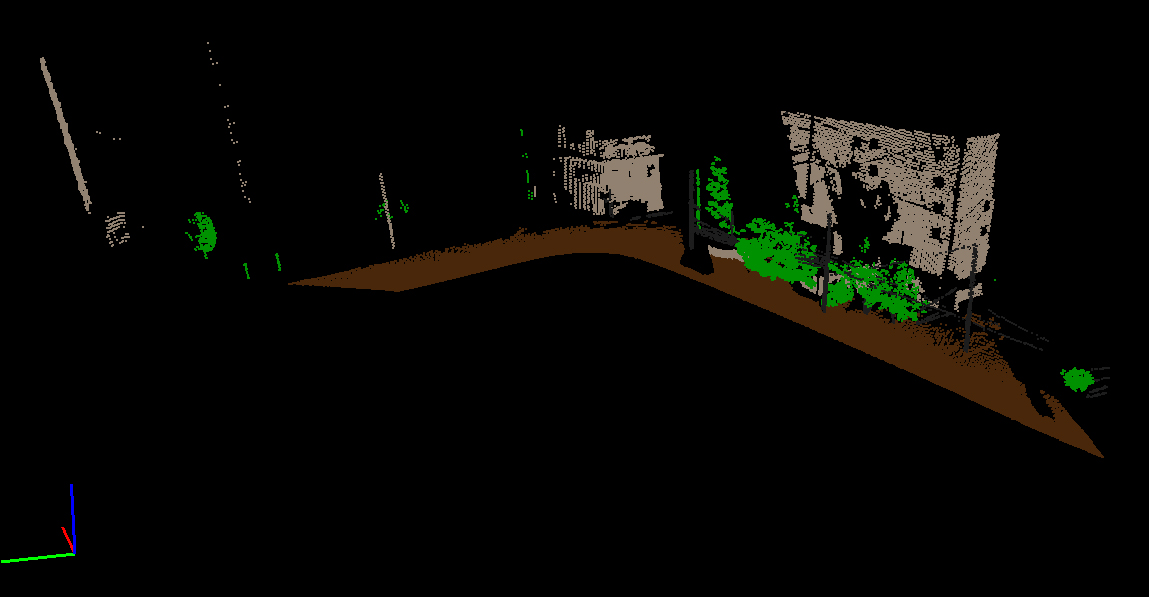
\includegraphics[scale = 0.3]{raw_cloud}
\caption{given data}
\end{figure}

\begin{figure}
  \centering
  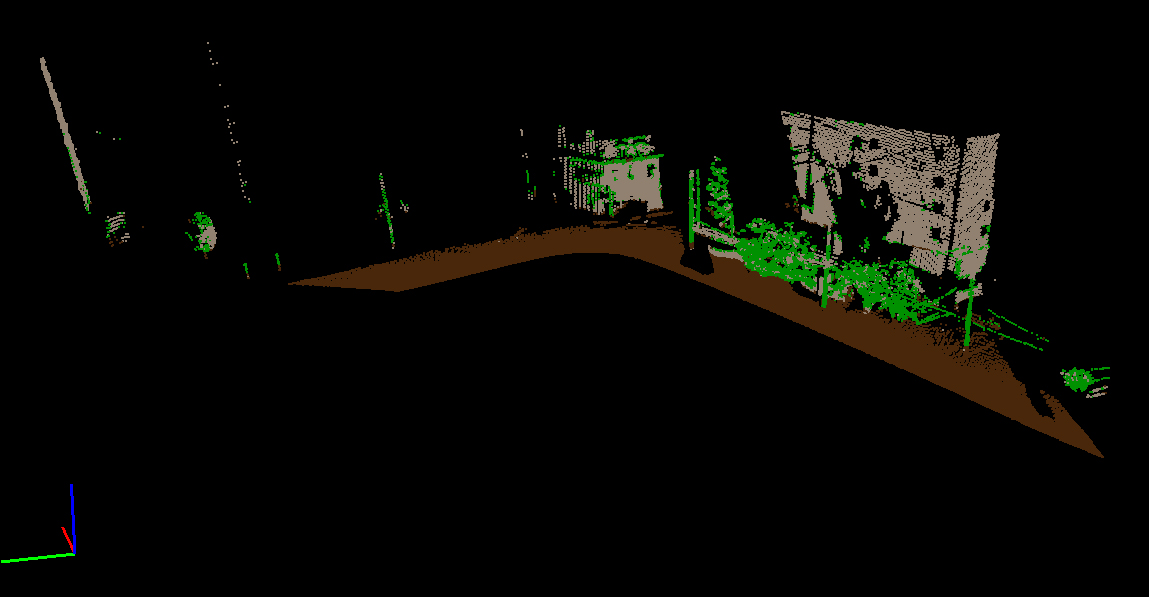
\includegraphics[scale = 0.3]{learned_cloud}
\caption{result from classification}
\label{fig:result from classification}
\end{figure}

 Here we showed classification after 10 passes of learning data. We see significant improvement by passing through the learning data twice when compared to passing it only once. There is however a little difference in classification performance when compare 10 passes learning versus 2 passes learning.

Wire and pole do not get classified very well for many potential reasons.








\end{document}
